\documentclass[a4paper 10pt]{article}
\usepackage[english,polish]{babel}
\usepackage[MeX]{polski}
\usepackage[utf8]{inputenc}
\usepackage[T1]{fontenc}
\usepackage[letterpaper, portrait, margin=1in]{geometry}
\usepackage{graphicx}
\usepackage{listings}
\usepackage{subfigure}
\usepackage{dashrule}
\usepackage{listings}
\usepackage{float}
\usepackage{amsmath}
\usepackage{listings}
\usepackage{multirow}
\usepackage{amsmath}
\usepackage{xcolor}
\usepackage{listings}
\usepackage{hyperref}
\hypersetup{ hidelinks = true, } 
\lstset{
    frame=single,
    breaklines=true,
    postbreak=\raisebox{0ex}[0ex][0ex]{\ensuremath{\color{red}\hookrightarrow\space}}
}


\renewcommand{\rmdefault}{ptm}
  
\frenchspacing

% Used to add additional dot in enumerations
\usepackage{titlesec}
\titlelabel{\thetitle.\quad}
\title{\textbf{Techniki Optymalizacji} \\
Laboratorium nr 2 \\
Sprawozdanie}
\author{Paulina Sadowska, Rafał Araszkiewicz}
\begin{document}
\maketitle

\section{Wprowadzenie}
Celem ćwiczenia było zaimplementowanie algorytmów rozwiązujących problem Komiwojażera dla zbioru 100 punktów. Algorytmy te znaleźć miały najbardziej optymalną ścieżkę łączącą 50 dowolnych punktów grafu gdzie punktem startowym miał być każdy z punktów znajdujących się w zbiorze. Dane testowe zawarte są na \hyperref[http://comopt.ifi.uni-heidelberg.de/software/TSPLIB95/XML-TSPLIB/instances/kroA100.xml.zip]{stronie Uniwersytetu Heidelberg}. 
\section{Local search}
\label{Local search}
W algorytmie tym trasa budowana jest w taki 
\subsection{Implementacja w pseudokodzie}
\begin{lstlisting}[frame=single]
dopoki zmiana trasy zmniejsza jej koszt

	dla kazdego z punktow na sciezce
		koszt = koszt przejscia do punktu i z punktu
		dla kazdego punktu spoza sciazki
			nowyKoszt = koszt przejscia do nowego punktu i z punktu
			jezeli nowyKoszt < najmniejszy z znalezionych nowych kosztow i nowyKoszt<koszt
				minKoszt = nowyKoszt
				
	dla kazdej pary punktow na sciezce
		dla kazdej kolejnej pary punktow na sciezce
			koszt = koszt przejscia miedzy para nr 1 + koszt przejscia miedzy para nr 2
			nowyKoszt = koszt przejscia miedzy pierwszymi punktami z kazdej z par + koszt przejscia miedzy drugimi punktami z kazdej z par
			jezeli nowyKoszt < najmniejszy z znalezionych nowych kosztow i nowyKoszt<koszt
				minKoszt = nowyKoszt			
	
	jezeli zysk z zamiany wierzcholkow jest wiekszy niz z zamiany krawedzi
		zamien punkt sciezki na ten dajacy lepszy zysk
	jezeli zmiana krawedzi przyniesie zysk	
		zamien  krawedzie miejscami
	w przeciwnym razie
		opusc petle
	
koniec

\end{lstlisting}
\label{Local search code}
\subsection{Wyniki}

%\begin{figure} [H]
%\centering
%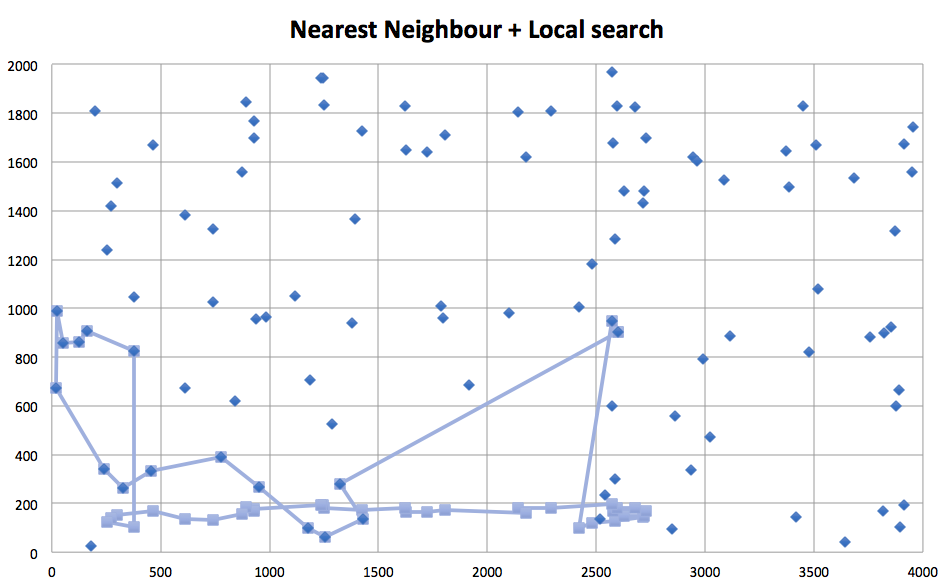
\includegraphics[angle=0,width = 1\textwidth, height=!]{images/NN.png}
%\caption{Najlepsza trasa - Nearest Neighbour}
%\label{Rys. NN}
%\end{figure}

\end{document}